\section{Methodische Vorgehensweise}

Der Forschungsbereich dieser wissenschaftlichen Abhandlung umfasst die Themengebiete CI/CD sowie Composable-Enterprise-Architekturen. Da in Kombination dieser beiden Forschungsbereiche sowie in der praktischen Umsetzung dieser Konzepte mit SAP-spezifischen Technologien in der Literatur kein Datenmaterial vorhanden ist, werden im Rahmen dieser Arbeit Experteninterviews durchgeführt. Die in diesen Gesprächen erhobenen Daten sollen dabei als Entscheidungsgrundlage zur Durchführung des AHP-Verfahrens verwendet werden.
\subsection{Semistrukturierte Leitfadeninterviews}
Das Experteninterview stellt eine häufig angewandte Analysemethode dar, welche vorrangig bei qualitativen Untersuchungen eines bestimmten Forschungsbereichs verwendet wird. Die Meinungen, Erfahrungen und Perspektiven der Experten werden dazu verwendete relevante Aspekte zu einem Thema zu identifizieren oder eine Forschungshypothese zu formulieren. Diese wissenschaftliche Methode wird dabei insbesondere für aktuelle stets unerforschte Themen sowie Fragestellungen mit geringem Literaturaufkommen verwendet. Als Experten werden in diesem Zusammenhang Interviewpartner bezeichnet, welche aufgrund ihres im Rahmen beruflicher Tätigkeiten erworbenen Wissens umfassende Kenntnisse in einem spezifischen Fachgebiet besitzen. Die konkrete Auswahl der Experten sollte in Abhängigkeit von Forschungsfrage sowie Evaluationsdesign erfolgen. So werden in der Literatur verschiedene Arten von Experteninterviews definiert. Dazu gehören strukturierte, semistrukturierte sowie unstrukturierte Interviews. Strukturierte Expertengespräche zeichnen sich dabei durch eine Vorabfestlegung der Fragen aus. Hierbei wird bezweckt, dass allen Teilnehmenden dieselben Fragen in standardisierter Reihenfolge vorgelegt werden. Deshalb eignen sich strukturierte Experteninterviews insbesondere für qualitative Datenerhebungen. Im anderen Extrem der unstrukturierten Interviews, wird Teilnehmenden eine Forschungsfrage definiert, jedoch keine expliziten Fragen festgelegt. Den konkreten Verlauf des Gespräches bestimmt dabei die dynamische Entwicklung des Antwort-Nachfrage-Verhaltens der Befragten bzw. des Interviewers. Da sich der Forschungsgegenstand dieser Abhandlung auf einen eng abgegrenzten Bereich bezieht, besteht bei unstrukturierten Experteninterviews das Risiko, dass die Gesprächsinhalte das Thema verfehlen. Eine Durchführung von strukturierten Interviews ist für diese Arbeit ebenfalls nicht geeignet. Das liegt insbesondere daran, dass das bei strukturierten Interviews vorhandene quantitative Erhebungsdesign nicht für die vorliegende Forschungsfrage geeignet ist. Vielmehr sollen im Verlauf dieser Abhandlung neue Themengebiete analysiert werden. Deshalb wurde sich für die Durchführung von semistrukturierte Interviews entschieden. Diese Interviewform realisiert eine allgemeine Leitdatenstruktur, welche essenziell zu behandelnde Fragen vorgibt, jedoch ebenfalls einen flexiblen Verlauf des Expertengesprächs ermöglicht. Diese Interviewform ist für die zugrundeliegende Arbeit besonders gut geeignet, da während des Gesprächs mit zusätzlichen Fragen auf bisher unbekannte Forschungsgebiete eingegangen werden kann. Der Interviewleitfaden sollte dabei sowohl offene als auch geschlossen Fragen beinhalten. Neben der Erzielung einer breiten Perspektive auf das zu untersuchende Thema ermöglicht dies ebenfalls spezifische Hypothesen zu validieren. Um die Interviews auswerten zu können muss eine Transkription der Gespräche vorgenommen werden. Dabei gibt es neben einer lautsprachlichen und einer vereinfachten ebenfalls eine zusammenfassende Transkription. Während in der lautsprachlichen Transkription die Inhalte des Gesprächs wortgetreu übernommen werden, werden Dialekte, Satzbrüche oder Wortdopplungen bei der vereinfachten Transkription nicht dokumentiert. Bei einer zusammenfassenden Transkription werden nur die wichtigsten Inhalte der des Interviews festgehalten. Da die Experteninterviews zur Erhebung von Daten zur Beantwortung der Forschungsfrage verwendet werden und dabei der genaue Wortlaut nicht essenziell ist, wird eine zusammenfassende Transkription durchgeführt. Zur tatsächlichen Auswertung wird dabei i.d.R. eine deduktive bzw. induktive Methode verwendet. Bei einer deduktiven Auswertung werden Aussagen der Experten bereits definierten Kategorien zugeordnet. Diese Evaluationsverfahren bietet dabei insbesondere zur Belegung einer vordefinierten Forschungshypothese einen großen Mehrwert. Da während dieser Arbeit lediglich eine offene Forschungsfrage beantwortet wird, wird eine induktive Kodierung der Interviews vorgenommen. Bei der induktiven Kodierung werden aus den Aussagen Kategorien abgeleitet und die Äußerungen der Experten sukzessive diesen Kategorien zugeordnet. Eine implizite Auswertung der induktiven Kodierung wird im AHP-Verfahren angewendet. So werden die während der Evaluation getroffenen Entscheidungen anhand der Expertenaussagen referenziert.

\subsection{Prototypische Implementierung der Integrations- und Bereitstellungs-Pipelines}

\subsection{Evaluation der Integrations- und Bereitstellungs-Pipelines unter Anwendung des Analytischen Hierarchieprozesses}
AHP ist ein Entscheidungs-Framework, welches von dem Mathematiker Thomas Saaty veröffentlicht wurde. Dieses Rahmenwerk eignet sich insbesondere für komplex strukturierte Entscheidungsprobleme. Bei AHP wird dabei ein Nutzen für anhand der Bewertung verschiedener Entscheidungsalternativen vorgenommen. Das Rahmenwerk basiert dabei auf der Annahme, dass für die unterschiedlichen Kritieren eine unterschiedliche Gewichtung vorgenommen wird. Das AHP wird insbesondere in komplexe betriebswirtschaftliche Problemstellungen verwendet. Dieses Rahmenwerk findet dabei insebsondere in der Technologieauswahl Anwendung. Hier müssen i.d.R. verschiedene Kritieren wie Kosten, Funktionalität oder Benutzerfreundlichkeit berücksichtigt werden. Dabei werden von verschiedenen Gewichtungen vorgenommen und anhand dessen ein Gesamtnutzwert für eine Technologie berechnet. Somit ermöglicht sich eine auf die Präferenzen des Entscheidungsträges abgestimmte Auswahl einer optimalen Technologie. Das AHP-Verfahren besteht dabei aus vier Schritten. Im ersten Schritt muss eine zu lösende Problemstellungen definiert werden. Anhand dessen werden verschiedene Entscheidungsalternativen ausgewählt. Um diese Entscheidungsalternativen zu beurteilen müssen verschiedene Bewertungskriterien festgelegt werden. Die Entscheidungsstruktur kann dabei belibig hierarchisch aufgebaut werden. So kann ein kann ein Kriterium in verschiedene Unterkriterien untergliedert werden. Auf höchster Ebene des AHP-Baums befindet sich dabei das Entscheidungsproblem. Die nächsten Hierarchieebenen enthalten dabei die Bewertungskriterien. Auf unterster Stufe befinden sich schließlich die Entscheidungsalternativen, welche im Hinblick auf auf die festgelegten Evaluationskriterien bewertet werden. Um eine auf die Präferenzen der Stakeholder angepasste Bewertung zu ermöglichen, müssen die zuvor festgelegten Entscheidungskriterien gewichtet werden. Besteht der AHP-Baum aus mehreren Stufen, muss die Gewichtung für jede Ebene getrennt durchgeführt werden. Dabei wird für jede Stufe zunächst isolierte Gewichtung vorgenommen. Um diese relative Wichtigkeit zu ermitteln wird ein paarweiser Vergleich der Bewertungskriterien durchgeführt. Hierbei wird evaluiert wie wichtig ein Kriterium gegenüber eines anderen ist. Die dabei durchgeführte Gewichtungsberwertung erfolgt auf einer Skala von 1 - 9. Dieses Intervall hat sich aufgrund empririscher Validierungen, als das für Anwender geeignetste Gewichtungsintervall etabliert. Während der Wert 9 impliziert, dass ein Entscheidungskriterium wesentlich wichtiger ist, wird mit dem Index 1 eine gleiche Gewichtung ausgedrückt. Auf der rechten Hälfte der Matrixdiagonale müssen jeweils die transponierten Werte angeben werden. 
\begin{center}
	\begin{figure}[H]
		\centering
		\scalebox{0.3}{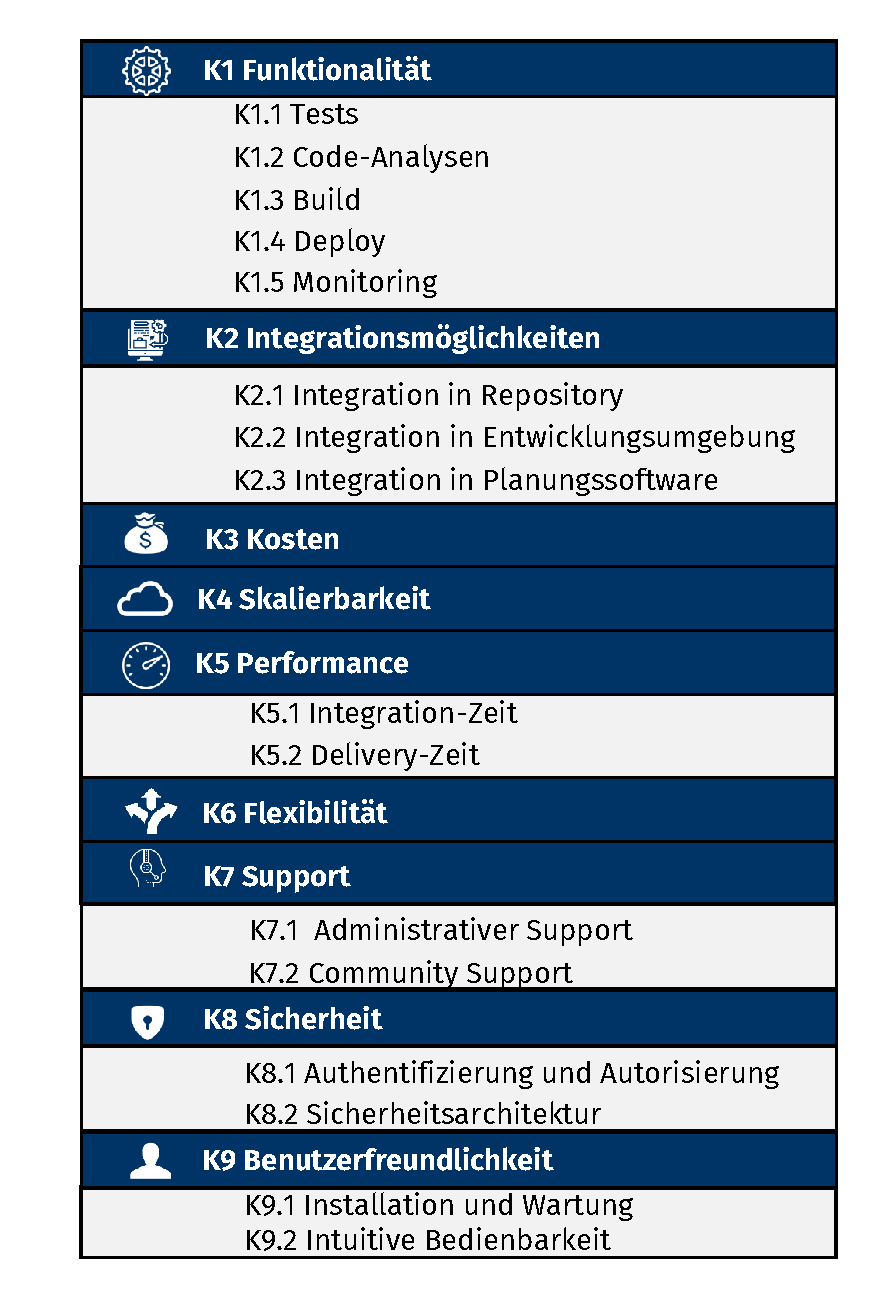
\includegraphics{AHP_B}}
		\caption[Exemplarische Darstellung der Paarvergleichsmatrix im AHP]{Exemplarische Darstellung der Paarvergleichsmatrix im AHP.\\ In Anlehnung an.}
		\label{fig:AHP_B}
	\end{figure}
\end{center}
\vspace*{-10mm}
So ist das in Abb. x dargestellte Kriterium x1 im Vergleich zu x2 7 mal so wichtig, während x2 im Vergleich zu x1 eine relative Wichtigkeit von 1/7 beträgt. Im dritten Schritt des AHP-Verfahrens wird die Ermittlung der prozentuale Gewichtung vorgenommen.
\begin{center}
	\begin{figure}[H]
		\centering
		\scalebox{0.3}{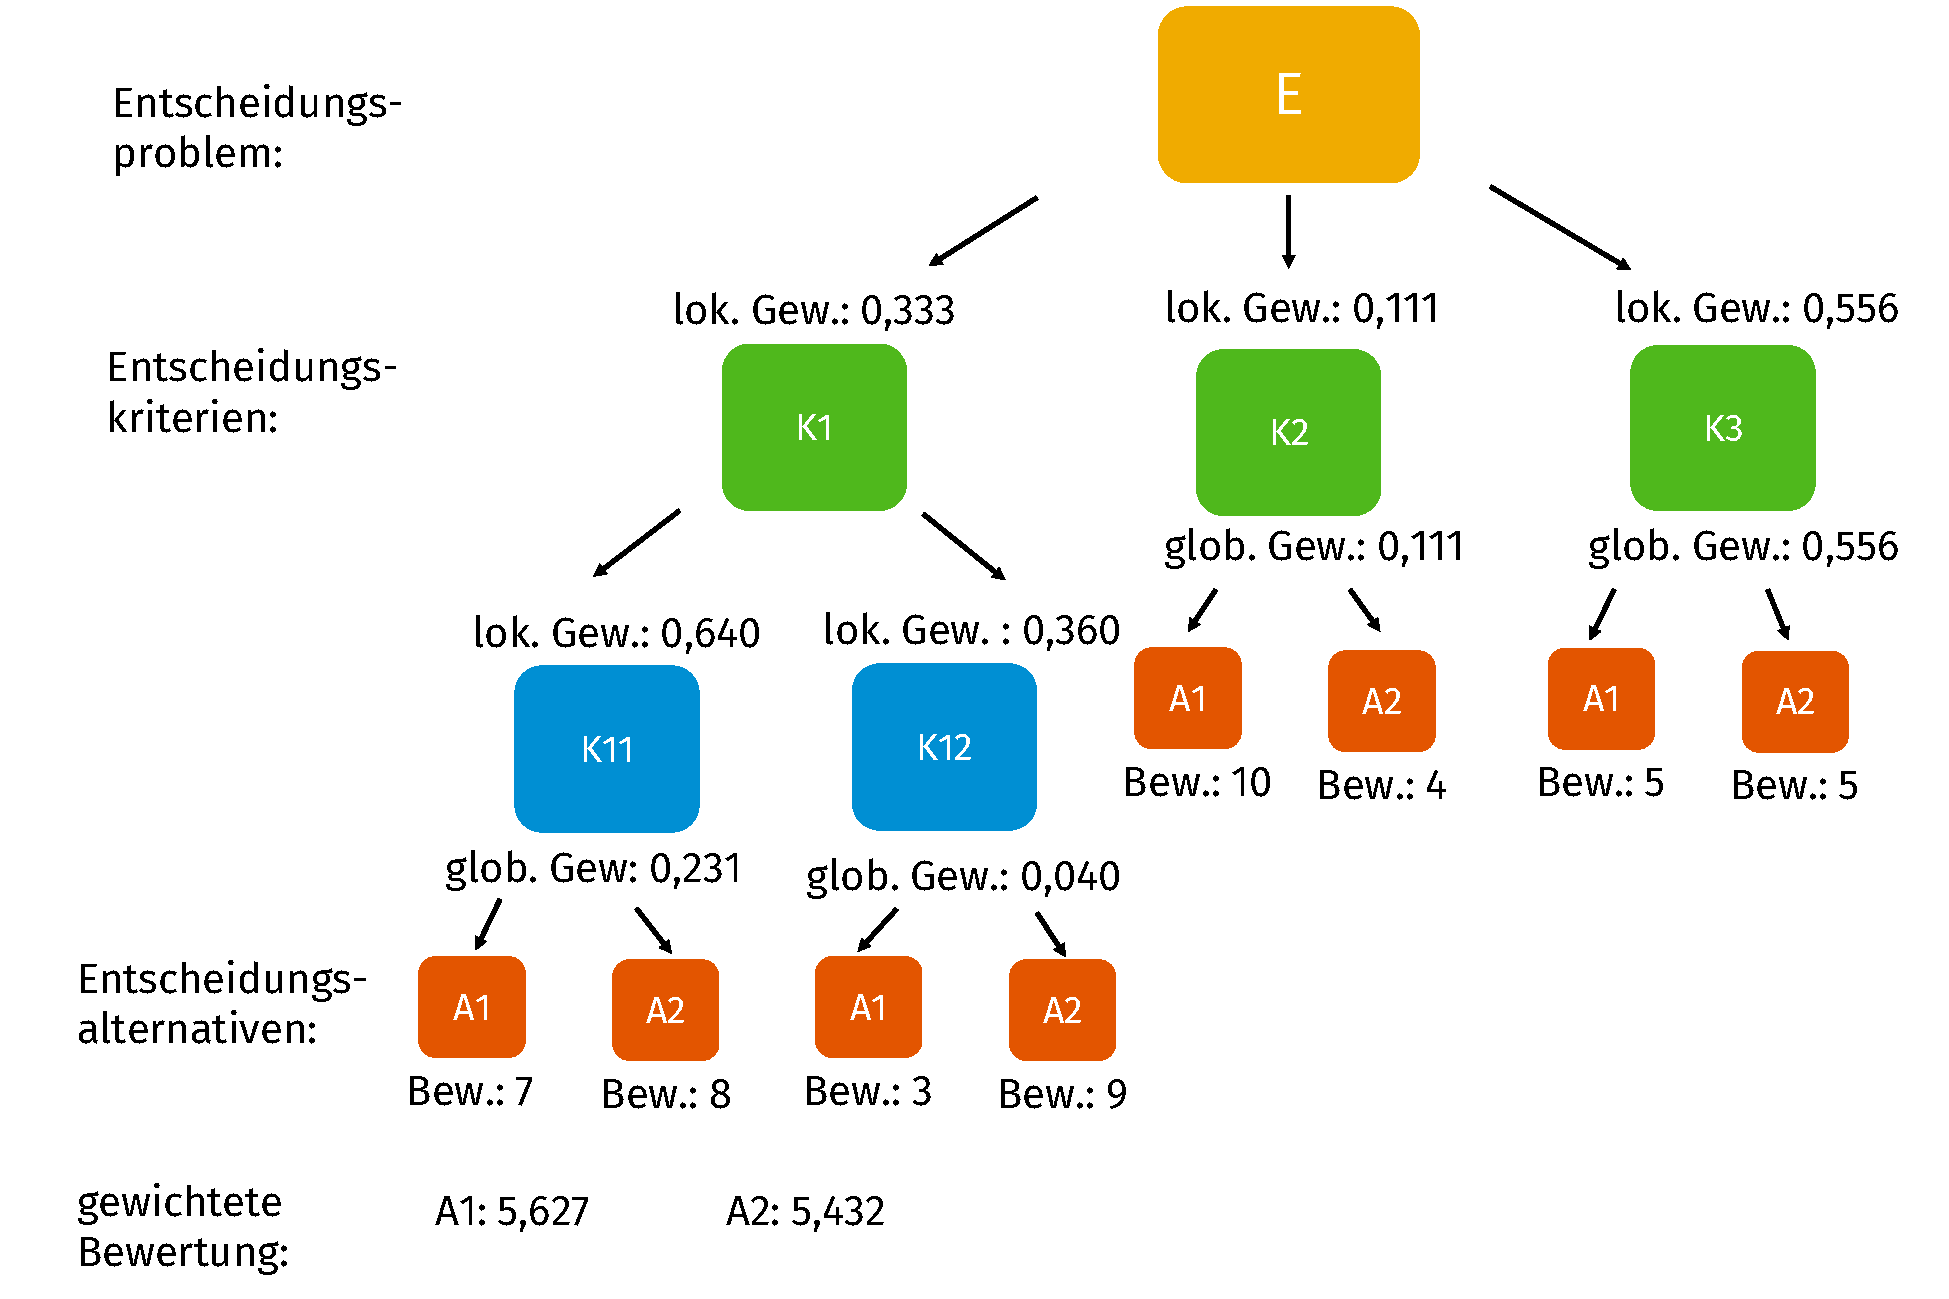
\includegraphics{AHP_H}}
		\caption[Exemplarische Darstellung der der hierarchischen Entscheidungsstruktur im AHP]{Exemplarische Darstellung der der hierarchischen Entscheidungsstruktur im AHP. In Anlehnung an.}
		\label{fig:AHP_B}
	\end{figure}
\end{center}
\vspace*{-10mm}
Hierbei wird zu die lokale Wichtigkeit ermittelt. Hierfür wird das auf der linearen Algebra basierende geometrische Mittel (\textit{v}) berechnet. Dafür werden zunächst die relativie Wichtigkeit einzelner Bewertungskriterien mutlipliziert. Aus dem Produkt wird im nächsten Schritt anschließend die n-te Wurzel gezogen. Um eine höhere Aussagekraft herzustellen muss dieser Dezimalwert normalisert werden. Dafür wird das geometrische Mittel eines Kriteriums durch die Summe aller geometrische Mittel dividiert. Damit wird sichergestellt, dass die Summe aller Gewichtungen 1 ist. Diese lokale Gewichtung wird für jede Stufe durchgeführt. Anschließend wird die Gewichtung jedes Unterkriteriums mit den Gewichtungen der oberen Kriterien mutlipliziert. Somit wird auf unterster Ebene, also bei dem Kriterium anhand welche eine Entscheidungsalternative letzlich bewertet wird, ein globales Gewicht berechnet. Entsprechend des Gesetzes der totalen Wahrscheinlichkeit ergeben alle globalen Gewichte in Summe den Wert 1. In der Literatur wird vorgesehen, dass auf unterster Hierarchieebene ebenfalls die Wichtigkeit der Entscheidungsalternativen gegeneinander abgewogen werden. Da dies insbesondere bei Entscheidungen mit persönlichen Präferenzen eine wichtige Rolle spielt, wird hierbei von dem Leitfaden nach Saaty abgewichen. Stattdessen wird für jedes Kriterium auf unterster Ebene eine feste Metrik von 0 - 1 definiert, anhand welcher die Alternativen bewertet werden. Letzlich werden diese Bewertung mit den globalen Gewichtungsfaktoren mutlipliziert und alle Noten einer Alternativen summiert. Die Alternative mit der höchsten gewichteten Gesamtberwertung gilt dabei als optimale Alternative. 

